PageRank is an algorithm for assessing the significance of nodes within a network by assigning numerical scores based on link structures \cite{rank-page99}. It operates on the principle that pages with more high-quality inbound links are of greater importance and thus should have higher ranks. While originally devised to rank web pages in search results, this metric finds applications in various domains, such as urban planning \cite{urban-zhang18}, video object tracking \cite{gong2013pagerank}, traffic flow prediction \cite{traffic-kim15}, dynamic asset valuation \cite{sawilla2006abstracting}, protein target identification \cite{banky2013equal}\ignore{, brain region importance assessment \cite{zuo2012network}}, software system characterization \cite{chepelianskii2010towards}, and identification of crucial species for environmental health \cite{allesina2009googling}\ignore{, and quantifying the scientific impact of researchers \cite{rank-senanayake15}}.

With the rise of extensive interconnected data, interest in parallel PageRank computation has surged. This has led to a number of implementations of parallel PageRank for multicore CPUs \cite{rank-garg16, rank-beamer17, rank-lakhotia18, grutzmacher2020acceleration, huang2020accelerating, chen2021hipa}. Unfortunately, multicore CPUs only offer a limited\ignore{parallelism and} memory bandwidth. This makes them unsuitable for graph algorithms, such as PageRank, which have a low computation-to-communication ratio. GPUs, on the other hand, boast extremely high bandwidth memory, connected in close proximity to thousands of lightweight cores with user-managed caches. Further, the GPU hardware is designed to be able to switch between running threads at no cost in order to support memory access latency hiding. When graphs algorithms are suitably designed, they can significantly outperform a parallel CPU-based implementation.

In recent years, significant research effort has focused on developing efficient parallel implementations of PageRank for GPUs \cite{duong2012parallel, rank-nvgraph, wang2016gunrock, busato2018hornet, dathathri2018gluon, nodehi2018tigr, grutzmacher2018high, piccinotti2019solving, grutzmacher2020acceleration, kang2020computing, wang2021grus, chen2022atos, chen2022scalable, yang2022graphblast, concessao2023meerkat}. These implementations, referred to as Static PageRank, compute ranks from scratch for a given graph, assuming the graph remains static over time. In this paper, we present our GPU implementation of Static PageRank, which utilizes a synchronous pull-based atomics-free computation method. It partitions and processes low and high in-degree vertices separately using two distinct kernels. Our implementation represents, to the best of our knowledge, the most efficient implementation for parallel PageRank computation on the GPU. Our GPU implementation of Static PageRank is compared with other state-of-the-art implementations in Table \ref{tab:compare-large}.\ignore{FPGAs \cite{rank-guoqiang20}, SpMV ASICs \cite{rank-sadi18}, CPU-GPU hybrids \cite{rank-giri20}, CPU-FPGA hybrids \cite{usta2020accelerating, rank-li21, rank-hassan21, rank-mughrabi21}, and distributed systems \cite{rank-sarma13, kang2022analyzing, vandromme2022scaling}.}

Real-world graphs often exhibit dynamic characteristics, undergoing frequent edge updates \cite{agarwal2012real, barros2021survey}. Recomputing PageRank scores for vertices upon each update, known as Static PageRank, can be resource-intensive. A strategy to reduce computation involves initiating PageRank computation from previous vertex ranks, thereby minimizing iterations required for convergence. We refer to this as the \textit{Naive-dynamic (ND)} approach. To further optimize runtime, recalculating ranks solely for potentially affected vertices is crucial. One common approach, which we refer to as the \textit{Dynamic Traversal (DT)} approach, entails identifying reachable vertices from updated graph regions and processing only those \cite{rank-desikan05, kim2015incremental, rank-giri20, sahu2022dynamic}. However, marking all reachable vertices as affected, even for minor changes, may lead to unnecessary computation, particularly in dense graph regions. Our previous work \cite{sahu2024df} addressed these concerns by introducing incrementally expanding \textit{Dynamic Frontier (DF)} and \textit{Dynamic Frontier with Pruning (DF-P)} approaches. These approaches process only a subset of vertices likely to change ranks, and were implemented as parallel multicore algorithms \cite{sahu2024df}. Here, we present our GPU implementation of DF-P PageRank, based on Static PageRank. It features partitioning between low and high out-degree vertices for incremental expansion of affected vertices using two additional kernels. Table \ref{tab:compare} shows the performance comparison of DF-P PageRank with Static, ND, DT, and DF PageRank.




\subsection{Our Contributions}

This technical report presents our improved Dynamic Frontier (DF) and Dynamic Frontier with Pruning (DF-P) approaches\footnote{\url{https://github.com/puzzlef/pagerank-cuda-dynamic}} for updating PageRank on dynamic graphs. These approaches efficiently identify vertices likely to change ranks upon batch updates, with minimal overhead. On a server with a 64-core AMD EPYC-7742 processor, our approaches outperform Static and Dynamic Traversal PageRank by $5.2\times$/$15.2\times$ and $1.3\times$/$3.5\times$ respectively on real-world dynamic graphs, and by $7.2\times$/$9.6\times$ and $4.0\times$/$5.6\times$ on large static graphs with random batch updates. Our observations indicate that the speedup offered by DF and DF-P PageRank mainly stems from the incremental marking of affected vertices. Additionally, our approaches show performance gains of $1.8\times$/$1.7\times$ for every doubling of threads.

\begin{table}[hbtp]
  \centering
  \caption{Speedup of our GPU implementation of Static PageRank compared to other state-of-the-art implementations. Direct comparisons are based on running the given implementation on our server, while indirect comparisons (denoted with a $*$) involve comparing results obtained by the given implementation relative to a common reference (Hornet/Gunrock).}
  \label{tab:compare-large}
  \begin{tabular}{|c|c||c|}
    \toprule
    \textbf{PageRank implementation} &
    \textbf{Published} &
    \textbf{Our Speedup} \\
    \midrule
    Hornet \cite{busato2018hornet} & 2018 & $31\times$ \\ \hline
    Gunrock \cite{wang2016gunrock} & 2016 & $5.9\times$ \\ \hline
    Galois with Gluon \cite{dathathri2018gluon} & 2018 & $448\times^*$ \\ \hline
    Tigr \cite{nodehi2018tigr} & 2018 & $40\times^*$ \\ \hline
    Grus \cite{wang2021grus} & 2021 & $7.2\times^*$ \\ \hline
    Atos \cite{chen2022atos} & 2022 & $7.6\times^*$ \\ \hline
    Multi-GPU Atos ($1$ GPU) \cite{chen2022scalable} & 2022 & $7.8\times^*$ \\ \hline
    Multi-GPU Atos ($4$ GPUs) \cite{chen2022scalable} & 2022 & $4.8\times^*$ \\ \hline
    GraphBLAST \cite{yang2022graphblast} & 2022 & $11\times^*$ \\ \hline
    Meerkat \cite{concessao2023meerkat} & 2023 & $18\times^*$ \\ \hline
  \bottomrule
  \end{tabular}
\end{table}

\begin{table}[hbtp]
  \centering
  \caption{Speedup of our GPU implementation of Dynamic Frontier with Pruning (DF-P) PageRank compared to other approaches of updating PageRank scores (on GPU), on real-world dynamic graphs (Table \ref{tab:dataset}), and on large static graphs with random batch updates (Table \ref{tab:dataset-large}), respectively.}
  \label{tab:compare}
  \begin{tabular}{|l||c|}
    \toprule
    \textbf{PageRank approach} &
    \textbf{Speedup of DF-P} \\
    \midrule
    Static \cite{rank-page99} & $2.1\times$, $3.1\times$ \\ \hline
    Naive-dynamic (ND) \cite{rank-page99, rank-zhang17} & $1.5\times$, $1.7\times$ \\ \hline
    Dynamic Traversal (DT) \cite{rank-desikan05, kim2015incremental, rank-giri20, sahu2022dynamic} & $1.8\times$, $13.1\times$ \\ \hline
    Dynamic Frontier (DF) \cite{sahu2024df} & $2.1\times$ $1.3\times$ \\ \hline
  \bottomrule
  \end{tabular}
\end{table}





%% - Use --- for a dash.
%% - Use ``camera-ready'' for quotes.
%% - Use {\itshape very} or \textit{very} for italicized text.
%% - Use \verb|acmart| or {\verb|acmart|} for mono-spaced text.
%% - Use \url{https://capitalizemytitle.com/} for URLs.
%% - Use {\bfseries Do not modify this document.} for important boldface details.
%% - Use \ref{fig:name} for referencing.

%% For a block of pre-formatted text: 
% \begin{verbatim}
%   \renewcommand{\shortauthors}{McCartney, et al.}
% \end{verbatim}

%% For a list of items:
% \begin{itemize}
% \item the ``ACM Reference Format'' text on the first page.
% \item the ``rights management'' text on the first page.
% \item the conference information in the page header(s).
% \end{itemize}

%% For a table:
% \begin{table}
%   \caption{Frequency of Special Characters}
%   \label{tab:freq}
%   \begin{tabular}{ccl}
%     \toprule
%     Non-English or Math&Frequency&Comments\\
%     \midrule
%     \O & 1 in 1,000& For Swedish names\\
%     $\pi$ & 1 in 5& Common in math\\
%     \$ & 4 in 5 & Used in business\\
%     $\Psi^2_1$ & 1 in 40,000& Unexplained usage\\
%   \bottomrule
% \end{tabular}
% \end{table}

%% For a full-width table:
% \begin{table*}
%   \caption{Some Typical Commands}
%   \label{tab:commands}
%   \begin{tabular}{ccl}
%     \toprule
%     Command &A Number & Comments\\
%     \midrule
%     \texttt{{\char'134}author} & 100& Author \\
%     \texttt{{\char'134}table}& 300 & For tables\\
%     \texttt{{\char'134}table*}& 400& For wider tables\\
%     \bottomrule
%   \end{tabular}
% \end{table*}


%% For inline math:
% \begin{math}
%   \lim_{n\rightarrow \infty}x=0
% \end{math},

%% For a numbered equation:
% \begin{equation}
%   \lim_{n\rightarrow \infty}x=0
% \end{equation}

%% For an unnumbered equation:
% \begin{displaymath}
%   \sum_{i=0}^{\infty} x + 1
% \end{displaymath}

%% For a figure:
% \begin{figure}[h]
%   \centering
%   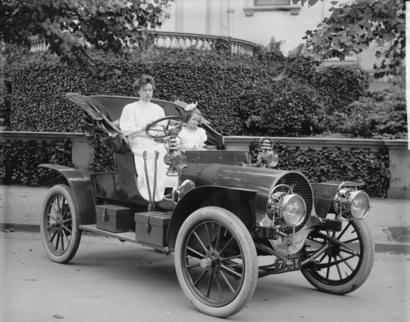
\includegraphics[width=\linewidth]{inc/sample-franklin}
%   \caption{1907 Franklin Model D roadster. Photograph by Harris \&
%     Ewing, Inc. [Public domain], via Wikimedia
%     Commons. (\url{https://goo.gl/VLCRBB}).}
%   \Description{A woman and a girl in white dresses sit in an open car.}
% \end{figure}

%% For a teaser figure.
% \begin{teaserfigure}
%   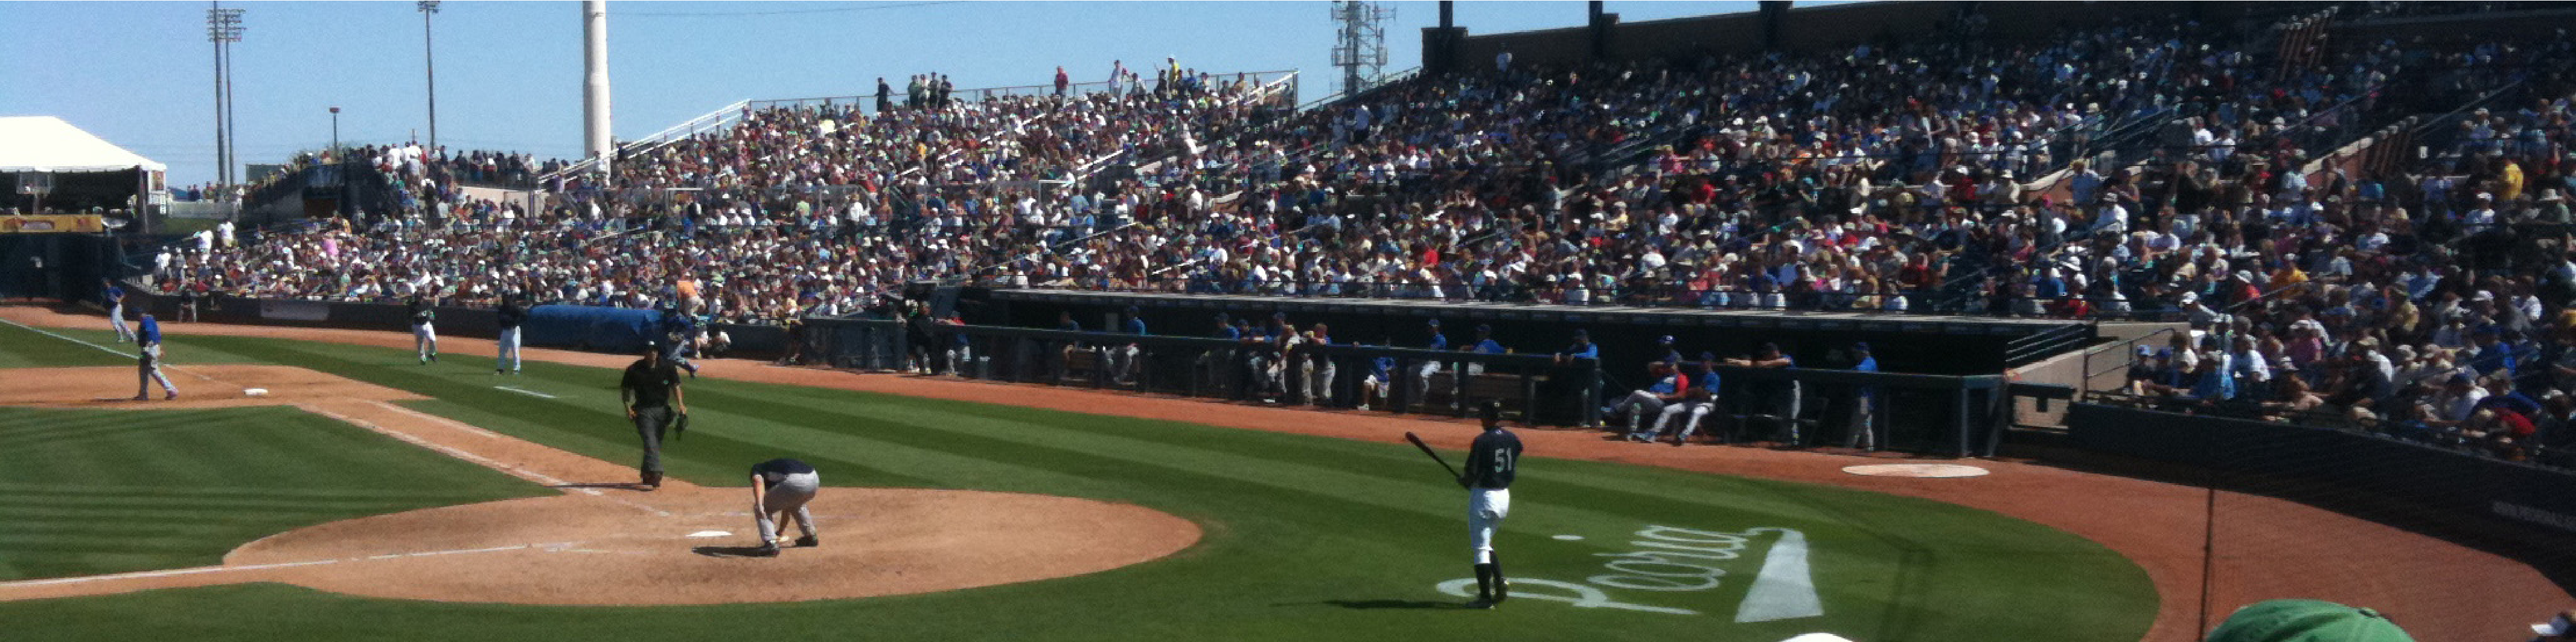
\includegraphics[width=\textwidth]{sampleteaser}
%   \caption{figure caption}
%   \Description{figure description}
% \end{teaserfigure}
